\title{Prediction, Bootstrapping and Monte Carlo Analyses Based on Linear Mixed Models with QAPE 2.0 Package}
\author{by Alicja Wolny--Dominiak and Tomasz \.{Z}\c{a}d{\l}o}

\maketitle             % Produces the title.

%\bigskip
%\abstract{
	%An abstract of less than 150 words.
	
	
	%Introductory section which may include references in parentheses
	%\citep{R}, or cite a reference such as \citet{R} in the text.
	
	%\section{Introduction}
	%\begin{figure}[htbp]
	%  \centering
	%  
\includegraphics{Rlogo}
	%  \caption{The logo of R.}
	%  \label{figure:rlogo}
	%\end{figure}
	
	%\section{Introduction}
	
	
	% Please keep the abstract below 300 words
	
	\abstract{
	The paper presents a new R package \CRANpkg{qape} for prediction, accuracy estimation of various predictors and Monte Carlo simulation studies of properties of both predictors and estimators of accuracy measures. It allows to predict any population and subpopulation characteristics of the response variable based on the Linear Mixed Model (LMM). The response variable can be transformed, e.g. to logarithm and the data can be in the cross-sectional or longitudinal framework. Three bootstrap algorithms are developed: parametric, residual and double, allowing to estimate the prediction accuracy. Analyses can also include Monte Carlo simulation studies of properties of the methods used. Unlike other packages, in the prediction process the user can flexibly define the predictor, the model, the transformation function of the response variable, the predicted characteristics and the method of accuracy estimation.
%
% 	\bigskip
% \noindent \textbf{Keywords:} linear mixed model, prediction accuracy, bootstrap procedures, model misspecification, Monte Carlo analyses
}

\section{Introduction}
\label{intro}
One of the tasks in application of mixed models in the real-life problems is the prediction of random effects. Then, the predicted values give the possibility for further prediction, e.g.  characteristics of interest such as sum, mean or quantiles or the future value of the response variable for cross-sectional or  longitudinal data.

Three main predictors of these characteristics are proposed in the literature: Empirical Best Linear Unbiased Predictors - EBLUPs (see e.g. \cite{henderson1950estimation} and \cite{royall1976linear}), PLUG-IN predictors (see e.g. \cite{boubeta2016empirical}, \cite{chwila2019properties}, \cite{hobza2016empirical}) and Empirical Best Predictors - EBPs (see e.g. \cite{molina2010small}).  Each assumes the LMM to model the response  variable.

The numerous successful applications of these three predictors for cross-sectional and longitudinal data can be found in the model approach in survey sampling, including the small area estimation. In paper \cite{fay1979estimates} the Authors introduce the prediction of the mean income for small places based on the special case of the LMM model called Fay-Herriot model and the EBLUP. The analysis of poverty is extended in many works, e.g. in \cite{molina2010small} and \cite{christiaensen2012}. In turn, in \cite{SAE1988} the Authors analyse the total crop areas based on survey and satellite data using EBLUPs. The proposed LMM model is known as the Battese-Harter-Fuller model. The predictors are also exploited in the subject of experience rating in non-life insurance, see \cite{frees1999} and \cite{buhlmann2005}, where the longitudinal data are under consideration.  The insurance premium for the next period for every policy in the insurance portfolio is predicted.

A major challenge in this type of prediction is the estimation of the prediction accuracy measure.  Most often it is the Root Mean Squared Error (RMSE), which is given in analytical form or can be e.g. estimated using bootstrap. A feature of the distribution of the squared prediction error is usually a very strong positive asymmetry. Because the mean is not recommended as the appropriate measure of the central tendency in such distributions, the alternative prediction accuracy measure called the Quantile of Absolute Prediction Errors (QAPE), proposed by \cite{zadlo2013parametric} and \cite{zadlo2020bootstrap}, can be applied.

There is a variety of R packages to calculate the considered predictors together with the accuracy measure of prediction, usually the RMSE. The package \CRANpkg{sae}, see \cite{sae}, provides EBLUPs based on Fay-Herriot and Battese-Harter-Fuller models. In turn, the multivariate EBLUP for Fay-Herriot models is implemented in \CRANpkg{msae}, see \cite{msae}. Several EBLUPs introduced in \cite{rao1994small} are implemented in package \CRANpkg{saery} introduced by \cite{saery}, likewise in \CRANpkg{JoSAE}, see \cite{josae}, but with additional heteroscedasticity analysis. The EBP is provided in the package \CRANpkg{emdi} described in \cite{kreutzmann2019r}.

 A new package in this area is our proposed package \CRANpkg{qape}.  It allows the prediction of flexibly defined characteristics of the response variable using the above three predictors, assuming an appropriate LMM. A novel feature of the package \CRANpkg{qape}, compared to those already in place, is the ability of bootstrap estimation of the prediction accuracy measures, both the RMSE and QAPE.  Three types of bootstrap procedures are provided: parametric, residual and double.

%The functions provided in the package \CRANpkg{qape} can be seen as giving an extension of some usability of all these packages.
There are three groups of functions in this package: predictors values calculation, bootstrap estimation of RMSE and QAPE measures, and Monte Carlo (MC) analysis of properties of predictors and prediction accuracy estimators. The prediction is based on a LMM model defined by the user and allows to predict the population characteristics of the response variable, which can be defined by a linear combination (in the case of EBLUP), by any R function (e.g. \code{sum}) or any function defined by the user (in the case of the EBP and PLUG-IN predictors). The package allows for full flexibility in defining: the model, the predicted characteristic, and the transformation of the response variable.

This paper is organized as follows. Firstly, the background of the LMM is presented together with the theoretical foundations of the prediction including prediction accuracy measures. Then, the package functionality in the area of prediction is presented and illustrated. A short application based on \code{radon} data, a cross-sectional dataset available in \CRANpkg{HLMdiag} package, to predict three subpopulation characteristics is shown. Subsequently, the theoretical background of the prediction accuracy measures estimation based on bootstrap is presented. Implementations of bootstrap algorithms in \CRANpkg{qape} are briefly introduced. Finally, the procedure of the model-based Monte Carlo simulation study is discussed. The paper ends with a conclusion.


\section{Prediction accuracy measures} \label{PAM}

We consider the problem of prediction of any given function of the population vector $\mathbf{Y}$ of the response variable:
\begin{equation}\label{theta}
\theta = f_{\theta}(\mathbf{Y})
\end{equation}
under the LMM. It covers linear combinations of $\mathbf{Y}$ (such as one future realization of the response variable or population and subpopulation means and totals) but also other population and subpopulation characteristics such quantiles and variability measures.


To assess the accuracy of the particular predictor $\hat \theta$, firstly, the prediction error is defined as $U=\hat{\theta}-\theta$. Therefore, the well-known RMSE has the following formula:
\begin{equation}\label{eq0}
	RMSE(\hat{\theta})=\sqrt{E(\hat{\theta}-\theta)^{2}}=\sqrt{E({{U}^{2}})}.
\end{equation}
The alternative to the RMSE based on the mean could be the QAPE based on quantiles. It represents the $p$th quantile of the absolute prediction error $|U|$, see \cite{zadlo2013parametric} and  \cite{zadlo2020bootstrap}, and it is given by:
\begin{equation}\label{eq1}
	QAPE_p(\hat{\theta}) = \inf \left\{ {x:P\left( {\left| {{\hat{\theta}-\theta}} \right| \le x} \right) \ge p} \right\} =\inf \left\{ {x:P\left( {\left| {{U}} \right| \le x} \right) \ge p} \right\}
\end{equation}
This measure informs that at least $p100\%$ of observed absolute prediction errors are smaller than or equal to $QAPE_p(\hat{\theta})$, while at least $(1-p)100\%$ of them are higher than or equal to $QAPE_p(\hat{\theta})$. Quantiles reflect the relation between the magnitude of the error and the probability of its realization. It means that using the QAPE, it is possible to make a full description of the distribution of prediction errors instead of using the average (reflected by the RMSE). Furthermore, the MSE is the mean of positively (usually very strongly) skewed squared prediction errors, where the mean should not be used as a measure of the central tendency of positively skewed distributions.

The above described accuracy prediction measures RMSE and QAPE can be estimated using the bootstrap techniques. Their estimators as well as the bootstrap distributions of the prediction errors based on any (assumed or misspecified) model are provided in \CRANpkg{qape} package, including algorithms where the parallel computing is used.

In the \CRANpkg{qape} package, the whole prediction process has its own specific procedure, which can be presented in the following steps.

\begin{procedure} The process of prediction, accuracy measures estimation and Monte Carlo simulation analyses in \CRANpkg{qape}
\label{Proc1}
\begin{enumerate}
    \item  Define the characteristics of the response variable to predict,
    \item  provide the information on sample and population values,
    \item  define the LMM,
    \item  estimate parameters of the LMM,
    \item  predict the random variable $\theta$ using the chosen class of predictors,
    \item  estimate the prediction accuracy measures RMSE and QAPE using one of the developed bootstrap algorithms,
    \item  conduct simulation analyses of properties of predictors and accuracy measures estimators under any (also misspecified) LMM model.
\end{enumerate}
\end{procedure}

\section{The prediction under LMM}

The main functions of the \CRANpkg{qape} package provide the bootstrap estimation of prediction accuracy measures. However, it must be preceded by the prediction process, including the choice of the LMM and the predictor.

\subsection{The model}
Let $\mathbf{Y}$ denote the vector of response variables $Y_1, Y_2,..., Y_N$. Assuming, without a loss of generality, that only the first $n$ realizations of $Y_i$ are observed, $\mathbf{Y}$ can be decomposed as $\mathbf{Y}=
\begin{bmatrix}
	\mathbf{Y}_s^T & \mathbf{Y}_r^T
\end{bmatrix}^T$ ,
where $\mathbf{Y}_s$ and $\mathbf{Y}_r$ are of dimension $n \times 1$ and $(N - n) \times 1$, respectively. In all notations, the subscript "s" is used for observed realizations of the variable of interest and "r" for the unobserved ones. Two known matrices of auxiliary variables are also considered, denoted by $\mathbf{X}$ and $\mathbf{Z}$, which are associated with fixed and random effects, respectively. The $\mathbf{X}$ matrix is of dimension $N \times p$, and it consists of $p$ regression variables. It can be decomposed like $\mathbf{Y}$ as follows: $\mathbf{X}=
\begin{bmatrix}
	\mathbf{X}_s^T & \mathbf{X}_r^T
\end{bmatrix}^T$,
where matrices $\mathbf{X}_s$ and $\mathbf{X}_r$, both known, are of dimension $n \times p$ and $(N-n) \times p$, respectively. Similarly, the $\mathbf{Z}$ matrix of dimension $N \times h$ can be written as follows: $\mathbf{Z}=
\begin{bmatrix}
	\mathbf{Z}_s^T & \mathbf{Z}_r^T
\end{bmatrix}^T$,
where matrices $\mathbf{Z}_s$ and $\mathbf{Z}_r$, both known, are of dimension $n \times h$ and $(N-n) \times h$, respectively.

Then, let $LMM(\mathbf{X}, \mathbf{Z}, \boldsymbol{\psi})$ denotes the LMM of the following form (e.g. \cite{rao2015small}, p. 98):
\begin{equation}
	\label{LMM}
	\left\{ \begin{array}{c}
		\mathbf{Y}=\mathbf{X}\boldsymbol{\beta} + \mathbf{Z}\mathbf{v}+\mathbf{e} \\
		E(\mathbf{e})=\mathbf{0}, E(\mathbf{v})=\mathbf{0} \\
		Var(\mathbf{e})=\mathbf{R}(\pmb{\delta}), Var(\mathbf{v})=\mathbf{G}(\pmb{\delta})
	\end{array} \right.
\end{equation}
The vector of parameters in model (\ref{LMM}) is then $\boldsymbol{\psi}=\begin{bmatrix}
	\boldsymbol{\beta}^T &  \pmb{\delta}^T
\end{bmatrix}^T$,
where $\boldsymbol{\beta}$ is a vector of fixed effects of dimension $p \times 1$ and $\pmb{\delta}$ is a vector of variance components. The random part of the model is described by the known matrix $\mathbf{Z}$, a vector $\mathbf{v}$ of random effects of dimension $h \times 1$ and a vector $\mathbf{e}$ of random components of dimension {$N\times 1$}, where $\mathbf{e}$ and $\mathbf{v}$ are assumed to be independent. The vector of random components $\mathbf{e}$ will be decomposed similarly to the vector $\mathbf{Y}$, i.e. $\mathbf{e}=\begin{bmatrix}
	\mathbf{e}_s^T & \mathbf{e}_r^T
\end{bmatrix}^T$.

In the residual bootstrap implemented in \CRANpkg{qape}, there is a need to re-write the LMM model to take account of the specific structure of data, i.e. the grouping variables taken into account in the random part of the model. In this case, without a loss of the generality, the LMM model can be written as follows:
\begin{equation}\label{LMMa}
	\mathbf{Y}=\mathbf{X}\boldsymbol{\beta} + \mathbf{Z}_1\mathbf{v}_1+...+\mathbf{Z}_l\mathbf{v}_l+...+\mathbf{Z}_L\mathbf{v}_L+\mathbf{e},
\end{equation}
where $\mathbf{v}_1,\dots,\mathbf{v}_l,\dots,\mathbf{v}_L$ are independent vectors of random effects assumed for different divisions of the $\mathbf{Y}$ vector (under different grouping of the data) and $\mathbf{Z}_1, \dots, \mathbf{Z}_l, \dots, \mathbf{Z}_L$ are known matrices of auxiliary variables associated with random effects. Writing in (\ref{LMMa}): $\mathbf{Z}=
\begin{bmatrix}
	\mathbf{Z}_1 & \dots & \mathbf{0} & \dots  & \mathbf{0} \\
	\vdots & \ddots &  &  & \vdots \\
	\mathbf{0} & \dots & \mathbf{Z}_l & \dots & \mathbf{0} \\
	\vdots &  &  & \ddots & \vdots \\
	\mathbf{0} & \dots & \mathbf{0} & \dots & \mathbf{Z}_L \\
\end{bmatrix}$ and
$\mathbf{v}=
\begin{bmatrix}
	\mathbf{v}_1^T & \dots & \mathbf{v}_l^T & \dots  & \mathbf{v}_L^T \\
\end{bmatrix}^T$
the LMM model is obtained. Let


\begin{equation} \label{vl}
\mathbf{v}_l=\left[ \mathbf{v}_{l1}^T \dots \mathbf{v}_{lk}^T \dots \mathbf{v}_{lK_l}^T \right]^T	
\end{equation}
be of dimension $K_l J_l \times 1$, where $\mathbf{v}_{lk}$ is of dimension $J_l \times 1$ for all $k=1,...,K_l$ and $K_l$ is the number of random effects at the $l$th level of grouping. Hence,  $\mathbf{Z}_l$ is $N \times K_l J_l$. For example, if the random regression coefficient model is considered with two random coefficients where both random effects are subpopulation-specific, where $D$ is the number of subpopulations, then $L=1$, $K_1=2$ and $J_1=D$.

\subsection{Predictors}
In the \CRANpkg{qape} package, in the general case the predicted characteristic  is given by any function of response variables:
\begin{equation} \label{ftheta}
\theta = f_{\theta}(\mathbf{Y}).
\end{equation}
Under the $LMM(\mathbf{X}, \mathbf{Z}, \boldsymbol{\psi})$ model it could be predicted using one of three predictors:
\begin{enumerate}
	\item Empirical Best Linear Unbiased Predictor (EBLUP),
	\item Empirical Best Predictor (EBP) under nested error LMM,
	\item PLUG-IN predictor under the LMM.
\end{enumerate}

The first predictor (EBLUP) allows to predict the linear combination of the response variables:
\begin{equation} \label{l.theta}
\theta = f_{\theta}(\mathbf{Y}) = \boldsymbol{\gamma}^T \mathbf{Y}= \boldsymbol{\gamma}_s^T \mathbf{Y}_s + \boldsymbol{\gamma}_r^T \mathbf{Y}_r,
\end{equation}
where $\boldsymbol{\gamma}$ is a vector of weights. In this case, the predicted characteristic $\theta$ is basically the linear combination of the response variable. For example, if one of the elements of $\boldsymbol{\gamma}$ equals 1 and the rest of the elements equals 0, then one realization of the response variable is predicted. If all elements in $\boldsymbol{\gamma}$ vector equal 1, then $\theta$ becomes the sum of all $Y_i$'s in the whole considered population dataset. The two-stage EBLUP corresponds to the Best Linear Unbiased Predictor (BLUP) introduced in \cite{henderson1950estimation} and \cite{royall1976linear} as:
\begin{equation} \label{BLUP}
	\hat{\theta}^{BLUP} (\pmb{\delta}) = {\boldsymbol{\gamma}}_s^T \mathbf{Y}_s  + \hat{\theta}_r(\pmb{\delta}),
\end{equation}
where the predictor of the linear combination $\boldsymbol{\gamma}_r^T \mathbf{Y}_r$ of unobserved random variables is given by $\hat{\theta}_r(\pmb{\delta})={\boldsymbol{\gamma }}_r^T {{\mathbf{X}}_r}{\tilde{\boldsymbol{\beta}} }(\pmb{\delta}) +\boldsymbol{\gamma }_r^T{\mathbf{Z}}_r{\mathbf{\tilde{v}}}(\pmb{\delta})$, where $\tilde{\boldsymbol{\beta}}(\pmb{\delta})$ is the Best Linear Unbiased Estimator of $\boldsymbol{\beta}$ and $\tilde{\mathbf{v}}(\pmb{\delta})$ is the Best Linear Unbiased Predictor of $\mathbf{v}$, both presented in (\ref{LMM}). As shown by \cite{zadlo2017EBLUP} p. 8094, if $Cov(\mathbf{e}_r, \mathbf{e}_s)=\mathbf{0}$, then the predictor (\ref{BLUP}) is the BLUP of $\theta$ defined as the linear combination (\ref{l.theta}). Even if $Cov(\mathbf{e}_r, \mathbf{e}_s) \neq \mathbf{0}$, the predictor $\hat{\theta}_r(\pmb{\delta})$ is the Best Linear Unbiased Predictor of the following linear combination of $\boldsymbol{\beta}$ and $\mathbf{v}$: ${\boldsymbol{\gamma }}_r^T{{\mathbf{X}}_r}{ {\boldsymbol{\beta}} } +\boldsymbol{\gamma }_r^T{\mathbf{Z}}_r{\mathbf{{v}}}$. The EBLUP $\hat\theta^{EBLUP}$ is obtained by replacing the vector of variance components $\pmb{\delta}$ in BLUP (\ref{BLUP}) with the estimator $\hat{\pmb{\delta}}$. If (a) the expectation of the predictor is finite, (b) $\hat{\pmb{\delta}}$ is any even, translation-invariant estimator of $\pmb{\delta}$, (c) the distributions of both random effects and random components are symmetric around $\mathbf{0}$ (not necessarily normal), the EBLUP remains unbiased, as proved by \cite{kackar1981unbiasedness}.

To introduce the second predictor, called EBP, considered e.g. by \cite{molina2010small}, firstly, the Best Predictor (BP) $\hat{\theta}^{BP}$ of characteristic $\theta(\mathbf{Y})$ has to be defined. It is computed by minimizing the Mean Squared Error $MSE(\hat\theta )=E(\hat\theta - \theta)^2$ and can be written as $\hat\theta^{BP} = E(\theta|\mathbf{Y}_s)$. It means that the conditional distribution of $\mathbf{Y}_r|\mathbf{Y}_s$ must be known to compute its value while at least the parameters of this distribution, denoted by $\boldsymbol{\psi}$ in (\ref{LMM}), are unknown. The EBP $\hat\theta^{EBP}$ is obtained by replacing these parameters with estimators $\hat{\boldsymbol{\psi}}$. Its value can be computed according to the Monte Carlo procedure presented in the supplementary document for this paper.

The last predictor is the PLUG-IN predictor defined as (e.g. \cite{chwila2019properties}):
\begin{equation}
	\hat{\theta}^{PLUG-IN}=\theta(\begin{bmatrix}
		\mathbf{Y}_s^T & \mathbf{\hat{Y}}_r^T
	\end{bmatrix}^T),
\end{equation}
where $\mathbf{\hat{Y}}_r$ is the vector of fitted values of unobserved random variables under the assumed model (any model specified by the statistician). Under the LMM and if the linear combination of $\mathbf{Y}$ is predicted, the PLUG-IN predictor is the EBLUP, but generally, it is not optimal. However, it was shown in simulation studies that it can have similar or even higher accuracy compared to empirical (estimated) best predictors, where the best predictors minimize the prediction mean squared errors (cf. e.g. \cite{boubeta2016empirical}, \cite{chwila2019properties}, \cite{hobza2016empirical}). Moreover, the PLUG-IN predictor is less computationally demanding than the EBP.

\subsection{Predictors in \CRANpkg{qape}}

To deal with the LMM model, the \CRANpkg{qape} package  uses the \code{lmer()} function from the \CRANpkg{lme4} package, see \cite{lme4}. Assuming (\ref{LMM}) and based on $\mathbf{Y}_s$, the vector of model parameters $\boldsymbol{\psi} = [\boldsymbol{\beta}^T, \pmb{\delta}^T]^T$ is estimated using the Restricted Maximum Likelihood Method (REML), known to be robust on non-normality, see e.g \cite{jiang1996reml}, and $\hat{\boldsymbol{\psi}}$ is obtained.

In order to obtain the predictor of $\theta$, one of the three \CRANpkg{qape} functions can be applied: \code{EBLUP()}, \code{ebpLMMne()} or \code{plugInLMM()}. Firstly, the characteristic of response variables of interest has to be defined. It is actually obvious for EBLUP, which can be used only to predict the population/subpopulation linear combination (e.g. the sum) by using the argument \code{gamma} equivalent to the population vector of weights $\boldsymbol{\gamma}$ in (\ref{l.theta}). For other two predictors, the EBP and the PLUG-IN, the input argument called \code{thetaFun} has to be given (see $f_{\theta}(.)$ in (\ref{ftheta})). Function \code{thetaFun} could define one characteristic or a vector of characteristics, for example:

\begin{example}
> thetaFun1 <- function(x) median(x)
> thetaFun2 <- function(x) c(sum(x), mean(x), sd(x))
\end{example}


Secondly, two groups of input arguments, common to all three predictors, has to be provided:
\begin{itemize}
	\item {group 1 - arguments defining the sample and the population}
	\begin{itemize}
		\item   \code{YS} - values of the dependent variable in the sample ($\mathbf{Y}_s$),
		\item	\code {reg} - the population matrix of auxiliary variables named in \code{fixed.part}, \code{random.part} and \code{division},
		\item	\code{con} - the population $0-1$ vector with $1$s for elements in the sample and $0$s for elements which are not in the sample,
	\end{itemize}
	\item {group 2 - arguments defining the model}
	\begin{itemize}
		\item	\code{fixed.part} - fixed-effects terms declared as in \code{lm4::lmer} function,
        \item \code{random.part} - random-effects terms declared as in \code{lm4::lmer} function,
		\item	\code{weights} - the population vector of weights.
	\end{itemize}
\end{itemize}
The weights make it possible to include heteroscedasticity of random components in the LMM.
		
In \code{EBLUP()} and \code{plugInLMM()} the random-effects terms of the LMM have to be declared as the input argument \code{random.part}. The form of the \code{ebpLMMne} predictor, in turn, requires defining in the \code{ebpLMMne()} function the so-called \code{division} argument instead of \code{random.part}. This input represents the variable dividing the population dataset into subsets, which are taken into account in the nested error linear mixed model with '\code{division}'-specific random components (presented in supplementary document for this paper).

In the process of prediction, it is often necessary to perform data transformation before estimating the model parameters. An example is the logarithmic scaling of the variable of interest. The \CRANpkg{qape} package offers the possibility for declaring the argument \code{backTrans} to conduct the data back-transformation. Hence, a very flexible solution is used which allows to use any transformation of the response variable such that the back-transformation can be defined. This argument (available in R or defined by the user function) should be the back-transformation function of the already transformed dependent variable used to define the model, e.g. for log-transformed \code{YS} used as the response variable:
\begin{example}
> backTrans <- function(x) exp(x)
\end{example}

The main output is the value of predictor \code{thetaP}. For each class of predictors, there are two S3 methods registered for existing generic functions \code{print} and \code{summary}. The full list of output arguments is presented in detail in the \code{qape-manual} file, cf. \cite{qape}.

\subsection{Radon data and the model}

In order to demonstrate the functionality of the package's main functions, in the following examples the \code{radon} dataset available in \CRANpkg{HLMdiag} package (\cite{HLMdiag}) is analyzed. It contains the results of a survey measuring radon concentrations in 919 owner-occupied homes in 85 counties of Minnesota (see Figure \ref{map}). A study was conducted in 1987-1988 by the Minnesota Department of Health, showing that indoor radon levels are higher in Minnesota compared to typical levels in the U.S. In the data, the response variable  \code{log.radon} (denoted in (\ref{radon.model}) by $log(Y_{ic})$) is the radon measurement in logarithms of picoCurie per liter. The independent variables, on the other hand, are: \code{uranium} ($x_{1ic}$) the average county-level soil uranium content, \code{basement} ($x_{2ic}$) the 0-1 variable indicating the level of the home at which the radon measurement was taken - 0 for basement, 1 for the first floor, and \code{county} (denoted by subscript $c$ in (\ref{radon.model})) is county ID.

\begin{figure}[h]
\centering
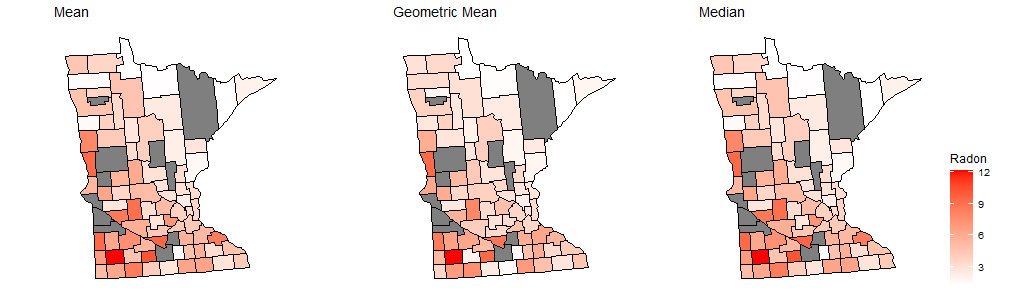
\includegraphics[scale=0.5]{mapaAll.png}
\caption{The maps of characteristics of radon concentration in counties in picoCurie per liter. The gray colour means that the value is NA (Not Available)}\label{map}
\end{figure}
In all considered examples, the prediction for the county no. 26 (\code{county == 26}) is conducted and it is assumed that the observations in this county from the first floor (\code{basement == 1}) are not available (see Figure \ref{boxplot}).

\begin{figure}[h]
\centering
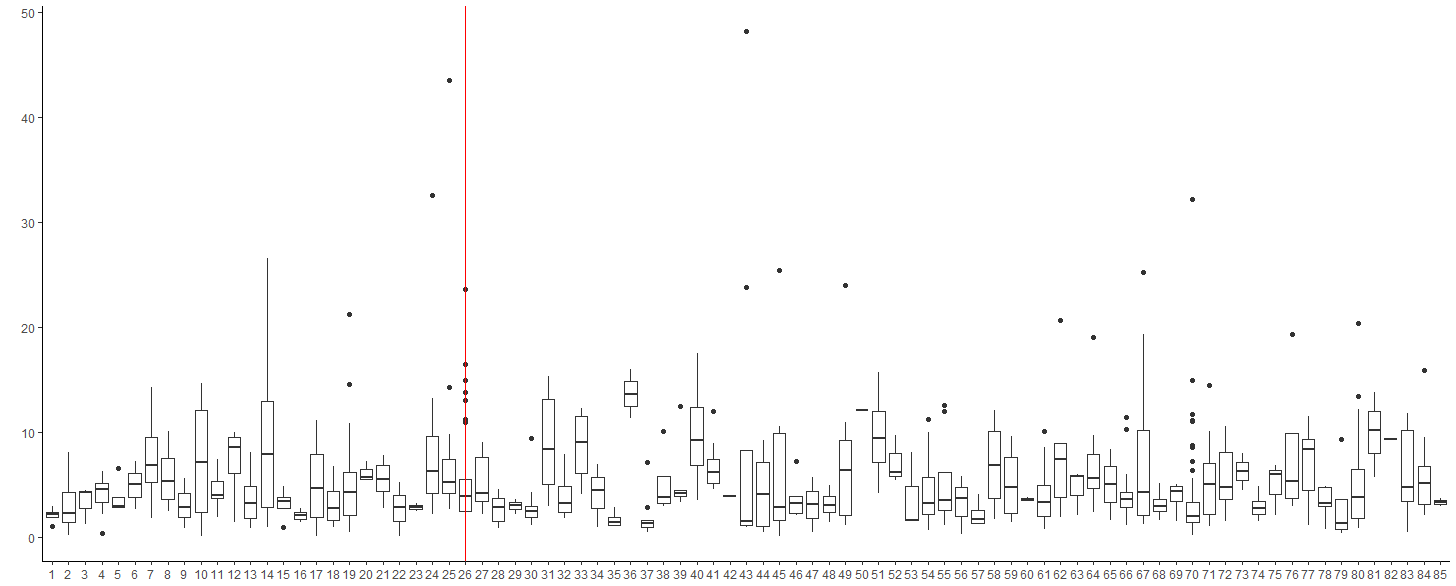
\includegraphics[scale=0.55]{boxAll.png}
\caption{The distributions of radon concentration in picoCurie per liter in counties. The red line indicates county no. 26}\label{boxplot}
\end{figure}
The \code{radon} dataset is widely discussed in the literature. In the paper \cite{nero1994statistically}, the Authors used an ordinary regression model to predict county geometric means of radon concentration using surficial soil radium data from the National Uranium Resource Evaluation. In turn, the paper \cite{price1996bayesian} focuses on the prediction of the geometric mean of radon for each county, but using a Bayesian approach. For the  \code{radon} data we use the following model
\begin{equation}\label{radon.model}
    log(Y_{ic}) = \beta_1 x_{1ic} + (\beta_2 + v_{1c}) x_{2ic} + \beta_0 + v_{2c} + e_{ic},
\end{equation}
where $i=1,2,\dots,N$, $c=1,2,\dots, C$, $N = 919$ observations, $C = 85$ counties, $\beta_1$, $\beta_2$ and $\beta_0$ are unknown fixed effects, $v_{1c}$ and $v_{2c}$ are random effects, $e_{ic}$ are random components, $v_{1c}$, and $e_{ic}$ are mutually independent, $v_{2c}$ and $e_{ic}$ are mutually independent too, $Cor(v_{1c}, v_{2c}) = \rho$, $v_{1c} \sim (0, \sigma^2_{v_1})$, $v_{2c} \sim (0, \sigma^2_{v_2})$  and $e_{ic} \sim (0, \sigma^2_e)$. As can easily be seen, the considered model is the random coefficient model with two correlated \code{county}-specific random effects. Its syntax written using the package \CRANpkg{lme4} notation is as follows:
\begin{verbatim}
radon.model <-	lmer(log.radon ~ basement + uranium + (basement | county), data = radon)
\end{verbatim}
This and similar LMMs are considered, analyzed, and used for the considered dataset in many publications, with a good overview presented in \cite{gelman_data_2006}. In \cite{gelman2006bayesian}, based on their preceding research \cite{price1996bayesian}, \cite{gelman1999analysis}, \cite{peck_should_2005}, a very similar model but with additional multivariate normality assumptions is studied, verified and chosen as fitting well to the data within a Bayesian framework. The same model as in \cite{gelman2006bayesian} with its special cases is considered in \cite{cantoni2021review} but within the frequentist approach. Based on 25 measures of explained variation and model selection, the Authors conclude that the same model as considered in our paper (with additional normality assumption, however, which is not used in all cases considered in that paper), "seems the best" \cite[p. 10]{cantoni2021review} for the \code{radon} data. Further tests of the model are presented by \cite{loy2013diagnostics}, \cite{loy2015you} and \cite{loy2017model} (see also \cite{cook2007interactive} for the introduction of the methodology) showing among others: the normality and homescedasticity of random components, the normality of the distribution of the random slope but – what is important for our further considerations – the lack of the normality of the random intercept. Since the problem of choosing and verifying a model for the considered dataset is widely discussed in the literature, we will focus on the issues that are new in this case, namely the problem of prediction and estimation of the prediction accuracy as well as the Monte Carlo analysis of predictors' properties.

\subsection{Example 1}

This example shows the prediction procedure in the package \CRANpkg{qape}. In the first step, it is needed to define all the input arguments that will then be passed to the prediction functions.
\begin{verbatim}
> Ypop <- radon$log.radon # the population vector of the dependent variable
> # It is assumed that observations from the first floor
> # in county no. 26 are not available:	
> con <- rep(1, nrow(radon))
> con[radon$county == 26 & radon$basement == 1] <- 0
> YS <- Ypop[con == 1] # sample vector of the dependent variable
> reg <- dplyr::select(radon, -log.radon) # the population matrix of auxiliary variables
> fixed.part <- 'basement + uranium' # the fixed part of the considered model
> random.part <- '(basement|county)' # the random part of the considered model
> # The vector of weights to define
> # the predicted linear combination -  the mean for county == 26:
> gamma <-
+   (1 / sum((radon$county == 26))) * ifelse((radon$county == 26), 1, 0)
> estMSE <- TRUE # to include the naive MSE estimator of the EBLUP in the output
\end{verbatim}

Then the functions corresponding to each predictor can be used. First,  the EBLUP prediction in the package \CRANpkg{qape} is presented.  As the EBLUP is limited to  the linear combination of random variables, the predicted characteristic is simply the arithmetic mean. To be precise, it is the mean of logarithms of measurements (instead of the mean of measurements), because the EBLUP can be used only under the linear (linearized) models. As in the LMM the homescedasticity of random components is assumed, the input argument \code{weights = NULL} is set up.

\begin{verbatim}
> myeblup <- EBLUP(YS, fixed.part, random.part, reg, con, gamma,  weights = NULL, estMSE)
> # the value of the predictor of the arithmetic mean
> # of logarithms of radon measurements:
> myeblup$thetaP
[1] 1.306916
> myeblup$neMSE # the value of the naive MSE estimator
[1] 0.002292732
\end{verbatim}
Hence, the predicted value of the arithmetic mean of logarithms of radon measurements equals $1.306916$ log picoCurie per liter. The estimated root of prediction MSE equals $\sqrt{0.002292732} \approx 0.048$ log picoCurie per liter, but -- what is important -- it is the value of the naive RMSE estimator \citep[as defined by][p. 106]{rao2015small}, which means that it ignores the decrease of accuracy due to the estimation of model parameters.

 The second part of this example shows the prediction of the arithmetic mean, geometric mean and median of radon measurements (not logarithm of radon measurements) in county no. 26 with the use of the PLUG-IN predictor. It requires the setting of two input arguments: \code{thetaFun} and \code{backTrans}.

\begin{verbatim}
> thetaFun <- function(x) {
+   c(mean(x[radon$county == 26]), psych::geometric.mean(x[radon$county == 26]),
+     median(x[radon$county == 26]))
+   }
> backTransExp <- function(x) exp(x) # back-transformation
> myplugin <- plugInLMM(YS, fixed.part, random.part, reg, con, weights = NULL,
+                     backTrans = backTransExp, thetaFun)
> # values of the predictor of arithmetic mean, geometric mean
> # and median of radon measurements:
> myplugin$thetaP
[1] 3.694761 4.553745 3.900000
\end{verbatim}
%Using the PLUG-IN predictor we are able to predict any characteristic of the variable of interest, taking into account any tranformation, because the back-transformation must be defined.
In this case  we can conclude that the predicted values of the aritmethmic mean, geometric mean and median in county no. 26 equal: $3.694761$, $4.553745$ and $3.9$ picoCurie per liter, respectively. The problem of prediction accuracy estimation will be discussed in the next sections of the paper.

The \CRANpkg{qape} package allows to use the Empirical Best Predictor (EBP) (see the supplementary document for this paper) as well.  It provides predicted values of any function of the variable of interest, as the PLUG-IN predictor. However, this requires stronger assumptions to be met. The EBP procedure available in \CRANpkg{qape} package is prepared under the assumption of the normality of the variable of interest after any transformation. However, in the case of the considered model for logarithms of radon measurements, the assumption is not met as we mentioned before based on the results presented in the literature. It can also be verified using \code{normCholTest} function (available in \CRANpkg{qape} package) as follows:
\begin{verbatim}
> normCholTest(radon.model, shapiro.test)$p.value
[1] 2.589407e-08
\end{verbatim}
Moreover, due to the fact of very time-consuming iterative procedure used to compute the EBP for the general case, in the \CRANpkg{qape} package the function \code{ebpLMMne} uses a very fast procedure working only for nested error Linear Mixed Models (see \cite{molina2010small}).

The prediction of any function of the random variables based on cross-sectional data has been considered. Its special case, not presented above but widely discussed in the econometric literature, is the prediction of one random variable, in this case a radon measurement for one non-observed owner-occupied home. Furthermore, the \CRANpkg{qape} package is also designed for prediction based on longitudinal data for current or future periods as shown in examples for the \code{EBLUP}, \code{plugInLMM} and \code{ebpLMMne} functions in the \code{qape-manual} file, cf. \cite{qape}.

\section{Bootstrap procedures}

The \CRANpkg{qape} package provides three main types of bootstrap algorithms: the parametric bootstrap, the residual bootstrap and the double-bootstrap.

The parametric bootstrap procedure is implemented according to \cite{gonzales2007} and \cite{gonzales2008} and could be described in the following steps:

\begin{enumerate}
	\item based on $n$ observations of the dependent and independent variables ($\mathbf{Y}_s$, $\mathbf{X}_s$ and $\mathbf{Z}_s$) estimate $\boldsymbol{\psi}$ to obtain the vector of estimates $\boldsymbol{\hat{\psi}}$,
	\item generate $B$ realizations $y_{i}^{*(b)}$ of $Y_{i}$, under the $LMM(\mathbf{X}, \mathbf{Z}, \hat{\boldsymbol{\psi}})$ and multivariate normality of random effects and random components obtaining\\
	$\mathbf{y}^{*(b)}=\begin{bmatrix}	
	y_{1}^{*(b)} & ... & y_{i}^{*(b)} &... & y_{N}^{*(b)}
	\end{bmatrix}^T$, where $i=1, 2, ... ,N$ and $b=1, 2, ... ,B$,
	\item decompose the vector $\mathbf{y}^{*(b)}$ as follows
	$\begin{bmatrix}
		\mathbf{y}_s^{*(b)T} & \mathbf{y}_r^{*(b)T}
	\end{bmatrix}^T$,
	\item	in the $b$th iteration ($b=1,2,...,B$)
	\begin{enumerate}
		\item compute the bootstrap realization $\theta^{*(b)}=\theta^{*(b)}(\mathbf{y}^{*(b)},\boldsymbol{\hat{\psi}})$ of random variable $\theta$,
		\item obtain the vector of estimates $\boldsymbol{\hat{\psi}}^{*(b)}$ using $\mathbf{y}_s^{*(b)}$ and compute the bootstrap realization of predictor $\hat{\theta}$ denoted by $\hat{\theta}^{*(b)}(\mathbf{y}_s^{*(b)},\boldsymbol{\hat{\psi}}^{*(b)})$ based on $LMM(\mathbf{X}, \mathbf{Z}, \boldsymbol{\hat{\psi}}^{*(b)})$,
		\item compute bootstrap realizations of prediction error $U^*$ denoted by $u^*$ and for the $b$th iteration given by:
		\begin{equation}\label{u*b}
			u^{*(b)}=\hat{\theta}^{*(b)}(\mathbf{y}_s^{*(b)},\boldsymbol{\hat{\psi}}^{*(b)})-\theta^{*(b)}
			(\mathbf{y}^{*(b)},\boldsymbol{\hat{\psi}}) =\hat{\theta}^{*(b)}-\theta^{*(b)},
		\end{equation}
	\end{enumerate}
	\item compute the parametric bootstrap estimators of prediction accuracy measures: RMSE and QAPE replacing prediction errors $U$ in (\ref{eq0}) and (\ref{eq1}) by their bootstrap realizations.
\end{enumerate}
	
Another possible method to estimate the prediction accuracy measures is the residual bootstrap. In what follows, we use the notation $srswr(\mathbf{A}, m)$ to indicate the outcome of taking a simple random sample with replacement of size $m$ of rows of matrix $\mathbf{A}$. If $\mathbf{A}$ is a vector, it simplifies to a simple random sample with replacement of size $m$ of elements of $\mathbf{A}$.

To obtain the algorithm of the residual bootstrap, it is enough to replace step 2 of the parametric bootstrap procedure presented above with the following procedure of the population data generation based on (\ref{LMMa}):
\begin{itemize}
	\item generate $B$ population vectors of the variable of interest, denoted by $\mathbf{y}^{*(b)}$ as
	\begin{equation}\label{LMMboot}
		\mathbf{y}^{*(b)}=\mathbf{X}\hat{\boldsymbol{\beta}} + \mathbf{Z}_1\mathbf{v}^{*(b)}_1+...+\mathbf{Z}_l\mathbf{v}^{*(b)}_l+...+\mathbf{Z}_L\mathbf{v}^{*(b)}_L+\mathbf{e}^{*(b)},
	\end{equation}
	where $\hat{\boldsymbol{\beta}}$ is an estimator (e.g. REML) of ${\boldsymbol{\beta}}$,
	$\mathbf{e}^{*(b)}$ is a vector of dimension $N \times 1$ defined as $srswr(col_{1 \leq i \leq n } \hat{{e}}_{i}, N)$, where $\hat{{e}}_{i}$ ($i=1,2,...,n$) are residuals, $\mathbf{v}^{*(b)}_l$ (for $1,2,...,L$) is the vector of dimension $K_l J_l \times 1$ built from the columns of the matrix:
	$srswr \left(
	\left[ \begin{array}{ccccc}
		\hat{\mathbf{v}}_{l1} &
		\dots &
		\hat{\mathbf{v}}_{lk} &
		\dots &
		\hat{\mathbf{v}}_{lK_l}
	\end{array}
	\right], J_l
	\right)$
of dimension $J_l \times K_l$, where $\hat{\mathbf{v}}_{lk}$ are estimates of elements of random effects vector (\ref{vl}).
	
\end{itemize}
The next 3–5 steps in this procedure are analogous to steps in the parametric bootstrap procedure.

In the above-described step, it can be seen that if more than one vector of random effect is assumed at the $l$th level of grouping, then the elements are not sampled with replacement independently. In this case, rows of the matrix formed by these vectors are sampled with replacement.

The residual bootstrap algorithm can also be performed with so-called "correction procedure". This procedure, which can improve the properties of the residual bootstrap estimators due to the underdispersion of the uncorrected residual bootstrap distributions, is presented in the supplementary document for this paper.

\section{Bootstrap in \CRANpkg{qape}}

Two bootstrap procedures are implemented in separate functions: \code{bootPar()} (the parametric bootstrap) and \code{bootRes()} (the residual bootstrap). According to the general Procedure \ref{Proc1}, the step preceding the bootstrap procedure in both functions is the definition of the predictor object. It must be one of the following: \code{EBLUP}, \code{ebpLMMne} or \code{plugInLMM}. This object has to be passed to \code{bootPar()} or \code{bootRes()} as the input parameter \code{predictor}. The other input parameters are intuitive: \code{B} - the number of bootstrap iterations and \code{p} - order of quantiles in the estimated QAPEs.

The additional input parameter in \code{bootRes()} is a logical condition called \code{correction}, which makes it possible to include an additional correction term for both random effects and random components, presented in the supplementary document for this paper, to avoid the problem of underdispersion of residual bootstrap distributions.

The main output values in both functions are basically the measures: \code{estRMSE} and \code{estQAPE} computed based on (\ref{eq0}) and (\ref{eq1}), respectively, where prediction errors are replaced by their bootstrap realizations. There is also the output \code{error} being the vector of bootstrap realizations of prediction errors, which is useful e.g. in in-depth analysis of the prediction accuracy and for graphical presentation of results. To estimate these accuracy measures, we use below the residual bootstrap with the correction procedure.

%As it was mentioned earlier, the estimation of model parameters in our package is made using \code{lmer()} function from the \CRANpkg{lme4} package. There are known situations, listed for example by \cite{lme4} p. 25 where convergence warnings are generated by this function due to the fact the the estimated variances of random effects are close to zero. This issues may occur where model parameters are estimated for small or medium-sized data sets, where complex variance-covariance are assumed or the number of levels in groups taken into account for random effects is small. We have not observed such issues in case of estimation of model parameters based on the original dataset required to compute values of the predictors in previous sections. However, in the case of bootstrapping or Monte Carlo situations the situation is more complex. It is due to the fact the based on the estimates of model parameters the values of the dependent variables are generated $B$ times and than model parameters are estimated in each iteration. Hence, at least in some iterations, the values of the dependent variable can be generated based on the Linear Mixed Model, where the variance of random effects is relatively close to zero. Then, estimates of model parameters will be obtained however, convergance warnings can occur. In such a case, there are at least two possible solutions. Firstly, we can discard iterations with warnings but it will imply that our dependent variable will not follow the assumed model, as we would like to, but its conditional version only with relatively high values of variances of random effects. Secondly, we can take into account all generated realizations despite convergance warnings if only the parameters can be estimated for all iterations. We use the second solution following the argument presented in \cite{lme4} p. 25 who write that "being able to fit a singular model is an advantage: when the best fitting model lies on the boundary of a constrained space".


%%%%%%%%%%%%%%%
As previously stated, our package utilizes the \code{lmer()} function from the \CRANpkg{lme4} package for estimating model parameters. However, this function has been known to generate convergence warnings in certain situations,  listed for example by \cite{lme4} p. 25, when the estimated variances of random effects are close to zero. Such scenarios may occur when models are estimated for smaller or medium-sized datasets, when complex variance-covariance structures are assumed, or when the grouping variable considered for random effects has only a few levels. Although we have not observed such issues estimating model parameters based on the original dataset required to compute values of the predictors in previous sections, bootstrapping or Monte Carlo simulations are more complex cases. This is because, based on the estimates of model parameters, the values of the dependent variables are generated $B$ times, and then model parameters are estimated in each out of $B$ iterations. Therefore, in at least some iterations, dependent variable values may be randomly generated giving realizations, where the variance of the random effect is relatively close to zero. As a result, estimates of model parameters can be obtained; however, convergence issues implying warnings may occur. In such cases, there are at least two possible solutions. The first option is to discard iterations with warnings, which would imply that the dependent variable would not follow the assumed model as required, but instead only its conditional version with relatively high values of variances of random effects. It will imply overdispersed bootstrap distribution of random effects, which will affect the bias of the bootstrap estimators of accuracy measures. The second option is to consider all generated realizations, despite convergence warnings, as long as the parameters can be estimated for all iterations. We opted for the latter solution, as argued in \cite{lme4} p. 25, who noted that "being able to fit a singular model is an advantage: when the best fitting model lies on the boundary of a constrained space".
%%%%%%%%%%%%%



\subsection{Example 2}

%%% 2024-02-22


The analyses presented in Example 1 are continued. We extend the previous results to include the issue of estimating the prediction accuracy of the considered predictors. The use of functions for this estimation primarily requires an object of class predictor, here  "myplugin".
\begin{verbatim}
> class(myplugin)
[1] "plugInLMM"
\end{verbatim}
The short chunk of the R code presents the residual bootstrap estimators of the RMSE (\code{estRMSE}) and the QAPE (\code{estQAPE}) of the PLUG-IN predictors (\code{plugin}) of previously analyzed three characteristics of radon measurements in county no. 26: the arithmetic mean, geometric mean and median. In this and subsequent examples we make the computations for relatively high number of iterations allowing, in our opinion, to get reliable results. These results are also used to prepare Figure \ref{hist}. However, the computations are time-consuming. The supplementary R file contains the same chunks of the code but the number of iterations applied is smaller in order to execute the code swiftly.
\begin{verbatim}
> # accuracy measures estimates based on
> # the residual bootstrap with the correction:
> B <- 500 # number of bootstrap iterations
> p <- c(0.75, 0.9) # orders of Quantiles of Absolute Prediction Error
> set.seed(1056)
> residBoot <- bootRes(myplugin, B, p, correction = TRUE)
> # values of estimated RMSEs of the predictor of three characteristics:
> # the arithmetic mean, geometric mean and median of radon measurements, respectively:
> residBoot$estRMSE
[1] 0.1848028 0.2003681 0.2824359
> # values of estimated QAPEs
> # (of order 0.75 in the first row, and of order 0.9 in the second row)
> # of the predictor of three characteristics:
> # the arithmetic mean, geometric mean and median of radon measurements,
> # in the 1st, 2nd and 3rd column, respectively:
> residBoot$estQAPE
         [,1]      [,2]      [,3]
75% 0.1533405 0.2135476 0.2908988
90% 0.2813886 0.3397411 0.4374534
\end{verbatim}

Let us concentrate on interpretations of estimators of accuracy measures for the predictor of the geometric mean, i.e. the second value of \code{residBoot\$estRMSE}, and values in the second column of \code{residBoot\$estQAPE}. It is estimated that the average difference between predicted values of the geometric mean  and their unknown realizations equals $0.2003681$ picoCurie per liter. Furthermore, it is estimated that at least $75\%$ of absolute prediction errors of the predictor of the geometric mean are smaller or equal to $0.2135476$ picoCurie per liter and at least $25\%$ of absolute prediction errors of the predictor are higher or equal to $0.2135476$ picoCurie per liter. Finally, it is estimated that at least $90\%$ of absolute prediction errors of the predictor of the geometric mean are smaller or equal to $0.3397411$ picoCurie per liter and at least $10\%$ of absolute prediction errors of the predictor are higher or equal to $0.3397411$ picoCurie per liter. The distributions of bootstrap absolute prediction errors with values of estimated RMSEs and QAPEs for the considered three prediction problems are presented in Figure \ref{hist}.


\begin{figure}[h]
\centering
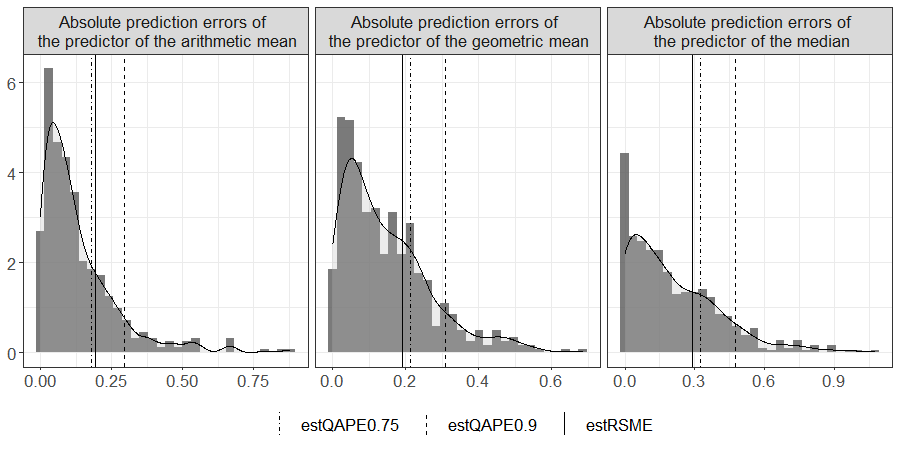
\includegraphics[scale=0.59]{histAll.png}
\caption{The histograms of bootstrap absolute prediction errors for \code{myplugin} (for PLUG-IN predictors of the arithmetic mean, geometric mean and median) for $B=500$}\label{hist}
\end{figure}



Since the assumption of normality is not met, the parametric bootstrap should not be used in this case. For this reason, we do not present the results for this method below, although -- but for illustrative purposes only -- they are presented in the supplementary R file. Moreover, these analyses can also be conducted using \code{bootParFuture()} and \code{bootResFuture()} functions where  parallel computing algorithms are applied. The input arguments and the output of these functions are the same as in \code{bootPar()} and \code{bootRes()}. Examples based on these functions are also included in the supplementary R file.

\section{Bootstrap under the misspecified model in \CRANpkg{qape}}
The \CRANpkg{qape} package also allows to use predictors under a model different from the assumed one (e.g. a simpler or more robust model), but estimate its accuracy under the assumed model. In this case, the parametric and residual bootstrap procedures are implemented in \code{bootParMis()} and \code{bootResMis()} functions. These functions allow to estimate the accuracy of two predictors under the model correctly specified for the first of them. Of course, it is expected that the estimated accuracy of the first predictor will be better than of the second one, but the key issue can be the difference between estimates of accuracy measures. A small difference, even to the second predictor's disadvantage, may be treated by the user as an argument for using the second predictor due to its properties, such as robustness or simplicity.

The considered functions allow to estimate the accuracy of two predictors, which belong to the class \code{plugInLMM}, under the model used to define the first of them. The remaining arguments are the same as in \code{bootPar()} and \code{bootRes()} functions: \code{B} - the number of bootstrap iterations, and \code{p} - orders of QAPE estimates to be taken into account.

The output results of \code{bootParMis()} and \code{bootResMis()} include -- similarly to \code{bootPar()} and \code{bootRes()} functions -- estimates of the RMSEs and QAPEs of both predictors (denoted here by: \code{estRMSElmm}, \code{estRMSElmmMis}, \code{estQAPElmm} and \code{estQAPElmmMis}), and boostrap realizations of their prediction errors (\code{errorLMM} and \code{errorLMMmis}).

\subsection{Example 3}

In this example, we study the same accuracy measures as in Example 2, but the aim is to compare the predictor \code{myplugin} and other predictor defined under the misspecified LMM. First, the misspecified model has to be defined, and a relevant predictor has to be computed.
\begin{verbatim}
> fixed.part.mis <- '1'
> random.part.mis <- '(1|county)'
> myplugin.mis <- plugInLMM(YS, fixed.part.mis, random.part.mis, reg, con,
+                         weights = NULL, backTrans = backTransExp, thetaFun)
\end{verbatim}
Having two objects: \code{myplugin} and \code{myplugin.mis}, one can proceed to a comparison by estimating bootstrap prediction accuracy performed using the residual bootstrap with correction procedure. In this case, we estimate the prediction accuracy of these two predictors under the model used to define the first of them.
\begin{verbatim}
> set.seed(1056)
> residBootMis <- bootResMis(myplugin, myplugin.mis, B, p, correction = TRUE)
> # residual bootstrap with the correction RMSE estimators
> # of 'plugin' of: arithmetic mean, geometric mean and median
> # of radon measurements in county 26:
> residBootMis$estRMSElmm
[1] 0.1848028 0.2003681 0.2824359
> # residual bootstrap with the correction RMSE estimators
> # of 'plugin.mis' of: arithmetic mean, geometric mean and median
> # of radon measurements in county 26:
> residBootMis$estRMSElmmMis
[1] 0.1919184 0.3192304 0.2762137
> # residual bootstrap with the correction QAPE estimators of order 0.75 and 0.9
> # of 'plugin' of: arithmetic mean, geometric mean and median
> # of radon measurements in county 26:
> residBootMis$estQAPElmm
         [,1]      [,2]      [,3]
75% 0.1533405 0.2135476 0.2908988
90% 0.2813886 0.3397411 0.4374534
> # residual bootstrap with the correction QAPE estimators of order 0.75 and 0.9
> # of 'plugin.mis' of: arithmetic mean, geometric mean and median
> # of radon measurements in county 26:
> residBootMis$estQAPElmmMis
         [,1]      [,2]      [,3]
75% 0.2267062 0.3802836 0.3255197
90% 0.2813787 0.4970726 0.4489399
\end{verbatim}

The results, presented above, were obtained for the same number of bootstrap iterations as in Example 2 ($B = 500$). If we compare, under the model defined in \code{plugin}, estimated RMSEs of \code{plugin} and \code{plugin.mis} predictors  of the geometric mean given by $0.2003681$ and $0.3192304$ picoCurie per liter, respectively, we can state that the estimated accuracy (measured by RMSE estimators) of the first predictor is better comparing with the second one. If we are not interested in the average accuracy measures but in the right tail of the distribution of prediction errors, we can use estimates of QAPE of order 0.9 to compare the accuracy. The result for the \code{plugin.mis} of the geometric mean equals to $0.4970726$ picoCurie per liter, and it is higher comparing with $0.3397411$ picoCurie per liter obtained for \code{plugin} for the same prediction problem. Hence, in this case, the accuracy comparison based both on the RMSE and QAPE leads to the same finding.

In the previous paragraph, we have focused on the results for the case of prediction of the geometric mean. If the comparison is made for the case of prediction of the arithmetic mean (the first column of output results) or the median (the third column of output results), we will come to the same conclusion regarding the estimated accuracy of \code{plugin} and \code{plugin.mis} as in the case of prediction of the geometric mean.

Similarly to the residual bootstrap, the parametric bootstrap procedure \code{paramBootMis} available in \CRANpkg{qape} package can be performed. However, in the considered case the normality assumption is not met (as discussed above) and the procedure is not recommended. The appropriate chunk of the R code is presented in the supplementary R file, but it is solely intended for illustrative purposes.

\section{Monte Carlo simulation analyses}

In the previous section, our aim was to estimate the prediction accuracy under correctly specified or misspecified model. In this section, we do not estimate the accuracy, but we approximate the true prediction accuracy under the specified model in the Monte Carlo simulation study. The crucial difference is that in this case, the model parameters used are obtained based on the whole population dataset, not the sample. If the number of iterations is large enough, we can treat the computed values of the measures as their true values, which are unknown in practice.

The last step of the analysis in \CRANpkg{qape} package presented in Procedure \ref{Proc1} is the Monte Carlo (MC) simulation analysis of:
\begin{itemize}
	\item properties of predictors
	\item and properties of parametric, residual and double bootstrap estimators of accuracy measures.
\end{itemize}
The whole Monte Carlo procedure is as follows.

\begin{procedure} Model-based Monte Carlo simulation analyses in \CRANpkg{qape}
\label{Proc2}
    \begin{enumerate}[label*=\arabic*.]
    	\item define the population vector of the dependent variable and the population matrix of auxiliary variables,
		\item provide the information on the division of the population into the sampled and non-sampled part,
		\item define $\theta$ - the characteristics of the response variable to be predicted,
		\item define the predictors $\hat{\theta}$ and accuracy measures estimators which properties are to be assessed,
		\item define the model to be used to generate realizations of the values of the dependent variable and estimate its parameters based on population data,
		\item For {k=1, 2, ..., K}
\begin{enumerate}[label*=\arabic*.]
		\item  generate the population vector of the response variable based on the assumed model,
		\item  based on population data, compute the characteristics $\theta$, denoted by  $\theta_k$,
		\item  based on sample data, estimate the parameters of the LMM,
		\item  based on sample data, compute values of predictors $\hat{\theta}$, denoted by  $\hat{\theta}_k$,
		\item  based on sample data, estimate the accuracy of $\hat{\theta}$ using bootstrap methods,
\end{enumerate}
 \item End For
	\item compute accuracy measures of predictors using $\hat{\theta}_k$ and $\theta_k$ (for $k=1,2, ..., K$),
	\item compute accuracy measures of estimators of prediction accuracy measures.
\end{enumerate}
\end{procedure}

\section{Monte Carlo analyses in \CRANpkg{qape}}

In order to perform a Monte Carlo (MC) analysis on the properties of predictors, it is necessary to have access to the entire population data for both dependent and independent variables. The function \code{mcLMMmis()} can be used with the following arguments. Firstly, the population values of the dependent variable (after a necessary transformation) should be declared as \code{Ypop}. By using the \code{Ypop} values, we can estimate the model parameters based on the entire population data (assuming that they are known). This allows us to generate values of the dependent variable in the simulation study that can mimic its distribution in the entire population, not just in the sample. This approach ensures that our simulation study can be an accurate representation of the random process in the entire population, resembling the real-world scenario. Secondly, three predictors: \code{predictorLMMmis}, \code{predictorLMM}, \code{predictorLMM2}, which belong to the class \code{plugInLMM}, are to be defined. The first one is used only to define the (possibly misspecified) model used to generate population values of the response variables. Accuracy of \code{predictorLMM} and \code{predictorLMM2} is assessed in the simulation study. The next two arguments include the number of MC iterations \code{K} and orders \code{p} of QAPEs used to assess the prediction accuracy. Finally, it should be noted that it is possible to modify covariance matrices of random components and random effects based on the model defined in \code{predictorLMMmis}, which are used tThiso generate values of the dependent variable. It is possible by declaring values of \code{ratioR} and \code{ratioG} arguments, which the diagonal elements of covariance matrices of random components and random effects, respectively, are divided by.

The output of this function covers the following statistics of both predictors computed in the simulation study: relative biases (\code{rBlmm} and \code{rBlmm2}), relative RMSEs (\code{rRMSElmm} and \code{rRMSElmm2}) and QAPEs (\code{QAPElmm} and \code{QAPElmm2}). Simulation-based prediction errors of both predictors (\code{errorLMM} and \code{errorLMM2}) are also taken into account.

\subsection{Example 4}

In the example, an MC simulation is carried out assuming the \code{myplugin} predictor. The goal is to  approximate  the true accuracy of the prediction assuming model (\ref{radon.model}). Hence, in the package \CRANpkg{qape},  all input predictor objects in the  function \code{mcLMMmis} have to be defined as  \code{myplugin}.
\
\begin{verbatim}
> # input arguments:
predictorLMMmis <- myplugin # to define the model
predictorLMM <- myplugin # which properties are assessed in the simulation study
predictorLMM2 <- myplugin  # which properties are assessed in the sim. study
\end{verbatim}
Except that no modification of covariance matrices has to be used.
\begin{verbatim}
# diag. elements of the covariance matrix of random components are divided by:
ratioR <- 1
# diag. elements of the covariance matrix of random effects are divided by:
ratioG <- 1
\end{verbatim}
We specify the number of Monte Carlo iterations.
\begin{verbatim}
K <- 500 # the number of MC iterations
\end{verbatim}
The analysis is conducted in the object \code{MC}.

\begin{verbatim}
> set.seed(1086)
> MC <- mcLMMmis(Ypop, predictorLMMmis, predictorLMM, predictorLMM2,
+                        K, p, ratioR, ratioG)
> # relative bias of 'predictorLMM'
> # of the arithmetic mean, geometric mean and median in county 26 (in %):
> MC$rBlmm
[1] -1.73208393 -0.04053178 -5.22355236
\end{verbatim}
Results of the relative biases are obtained. It is seen, that under the assumed model the values of the considered predictor of the geometric mean (the second value of \code{MC\$rBlmm}) are smaller than possible realizations of the geometric mean on average by $0.04053178\%$. In turn, the relative RMSEs are as follows.

\begin{verbatim}
> # relative RMSE of 'predictorLMM'
> # of the arithmetic mean, geometric mean and median in county 26 (in %):
> MC$rRMSElmm
[1] 3.429465 4.665810 7.146678
\end{verbatim}
In the considered case, the average difference between predicted values of the geometric mean and its possible realizations (the second value of \code{MC\$rRMSElmm}) equals $4.665810\%$. It should be noted that this value can be treated as the true value of the relative RMSE (if the number of iterations is large enough), not the estimated value obtained in Examples 2 and 3.

Finally, QAPEs of orders 0.75 and 0.9 are considered.
\begin{verbatim}
> # QAPE of order 0.75 and 0.9 of 'predictorLMM'
> # of the arithmetic mean, geometric mean and median in county 26:
> MC$QAPElmm
         [,1]      [,2]      [,3]
75% 0.1491262 0.1989504 0.2919221
90% 0.2895684 0.2959457 0.4728064
\end{verbatim}

Let us interpret the results presented in the second column of \code{MC\$QAPElmm}. At least $75\%$ ($90\%$) of absolute prediction errors of the predictor of the geometric mean are smaller or equal to $0.1989504$ ($0.2959457$) picoCurie per liter and at least $25\%$ ($10\%$) of absolute prediction errors of the predictor are higher or equal to $0.1989504$ ($0.2959457$) picoCurie per liter. Similar to the values of the rRMSEs in the previous code chunk, the values can be considered to be true QAPE values, not the estimates presented in Examples 2 and 3.

In Example 4, the accuracy of one predictor under the model used to define this predictor was presented. A more complex version of the simulation study, where the properties of two predictors are studied under the model defined by the third predictor, is presented in the supplementary R file. What is more, the \CRANpkg{qape} package also allows to use \code{mcBootMis()} function to conduct MC analyses of properties of accuracy measure estimators (estimators of MSEs and QAPEs) of two predictors (which belong to the class \code{plugInLMM}) declared as arguments. The model used in the simulation study is declared in the first predictor, but the properties of accuracy measures estimators of both predictors are studied. Output results of \code{mcBootMis()} covers simulation results on properties of different accuracy measures estimators, including the relative biases and relative RMSEs of the parametric bootstrap MSE estimators of both predictors. The same simulation-based statistics but for parametric bootstrap QAPE estimators are also included. Other bootstrap methods, including the residual bootstrap with and without the correction procedure, are also taken into account. The full list of output arguments of \code{mcBootMis()} function are presented in \code{qape-manual} file, cf. \cite{qape}.

\section{Conclusions}

The package enables R users to make predictions and assess the accuracy under linear mixed models based on different methods in a fast and intuitive manner -- not only based on the RMSE but also based on Quantiles of Absolute Prediction Errors. It also covers functions which allow to conduct Monte Carlo simulation analyses of properties of the methods of users interest. Its main advantage, compared to other packages, is the considerable flexibility in terms of defining the model (as in the \CRANpkg{lme4} package) and the predicted characteristic, but also the transformation of the response variable.

In our opinion, the package is useful for scientists, practitioners and decision-makers in all areas of research where accurate estimates and forecasts for different types of data (including cross-sectional and longitudinal data) and for different characteristics play the crucial role. We believe that it will be of special interest to survey statisticians interested in the prediction for subpopulations with small or even zero sample sizes, called small areas.


\bibliography{wolny-zadlo}


\address{Alicja Wolny--Dominiak\\
	Department of Statistical and Mathematical Methods in Economics \\
	University of Economics in Katowice\\
	 50, 1 Maja Street\\
	40--287 Katowice\\
	Poland\\}
\email{alicja.wolny-dominiak@uekat.pl} \\
\url{web.ue.katowice.pl/woali/}

\address{Tomasz \.{Z}\c{a}d{\l}o \\
Department of Statistics, Econometrics and Mathematics \\
University of Economics in Katowice\\
50, 1 Maja Street\\
40--287 Katowice\\
Poland\\}
\email{tomasz.zadlo@uekat.pl} \\
\url{web.ue.katowice.pl/zadlo/}

%\email{} \\

\end{article}

\end{document} 